\documentclass{thesisreport}

\setcounter{tocdepth}{3}
\setcounter{secnumdepth}{3}

\usepackage{caption}
\usepackage{subcaption}
\usepackage{comment}
\usepackage{amsmath}
\usepackage{bm}
\usepackage{multicol}
\usepackage{xcolor}
\usepackage{tabularx}
\usepackage{optidef}
\usepackage{mathtools}

\setlength{\columnseprule}{1pt}
\def\columnseprulecolor{\color{black}}
\DeclareUnicodeCharacter{2212}{-}

\setlength\parindent{0pt}

\begin{document}

 \thispagestyle{empty}

\def\lskip{\vspace{0.5cm}}


\begin{tabular}{p{7cm}p{8cm}}
ÉCOLE CENTRALE DE NANTES
&
% EMARO students only
% \raggedleft FIRST YEAR INSTITUTION	
\end{tabular}

\vspace{2cm}

% CORO-IMARO students
\begin{center} \large\sc MASTER CORO-IMARO\\ \normalsize{``CONTROL and ROBOTICS''} \end{center}

% EMARO students
%\begin{center} \large\sc MASTER ERASMUS MUNDUS \\ \normalsize{EMARO+ ``European Master in Advanced Robotics''} \end{center}


\begin{center}
	2020 / 2021\\
	\lskip
	Master Thesis Report %Master Thesis Report % or bibliography report
	\lskip
	
	Presented by \lskip 
	
	Elie Hatem \lskip
	
	On \today \lskip\lskip
	
	{\Large \textbf{Making Flips With Quadrotors In Constrained Environments}}
	
	\vfill

Jury \lskip
		
	\end{center}
	


\begin{tabular}{p{3cm}p{7cm}p{5cm} }
 % President: & Name & Position (Institution) \\ & & \\     % for final defense only (not bibliography)
 Evaluators: & Dr. Olivier Kermorgant & Associate Professor (ECN) \\
	      & Dr. Damien SIX & Robotics Engineer (CNRS) \\ 
	      %& Name & Position (Institution) \\ & & \\  & & \\ 
  Supervisor(s):  & Dr. Sébastien Briot & Researcher (CNRS) \\
		  & Dr. Isabelle Fantoni & Research Director (CNRS) \\
% EMARO students only
%(EMARO)  & Co-supervisor from M1 & Position, M1 institution 
\end{tabular}

\lskip

\begin{flushleft}
 Laboratory: Laboratoire des Sciences du Numérique de Nantes LS2N
\end{flushleft}

\newpage
\thispagestyle{empty}
\null
\newpage
\addtocounter{page}{-1}
\pagestyle{fancy}
  
 
  \section*{Abstract}
   
Within the rapidly growing aerial robotics market, one of the most substantial challenges in the quadrotor community is performing aggressive maneuvers, especially multi-flip maneuvers.  A proper physical definition of the issue is not addressed by the current approaches in the field and several key aspects of this maneuver are still overlooked.
It can be shown, in particular, that making a flip with a quadrotor means crossing the parallel singularity of the dynamic model. The aim of the master thesis is to explore the possibility of defining aggressive trajectories for quadrotors on the basis of their dynamic model degeneracy analysis and to adapt various strategies to control the robot in a closed loop. In addition, the possibility of performing the aggressive maneuvers in constrained environments will also be investigated.
Therefore, the analysis will be extended from the previous studies to create general feasible trajectories that will allow quadrotors to perform aggressive multi-flip maneuvers while passing through a constrained environment and while guaranteeing a satisfactory degree of robustness to the uncertainties of the dynamic model.\\

\textbf{Keywords: quadrotors, parallel robots, aggressive maneuvers, multi-flips, constrained environmen. }
 
 
 \newpage
 
 \section*{Acknowledgements}
 
 I would like to express my special thanks and gratitude to my supervisors Dr. Sébastien Briot and Dr. Isabelle Fantoni who gave me the  opportunity to work on this wonderful project which encapsulates control theory, dynamics and quadrotors, which are all subjects that are very interesting for me. 
This project has allowed me to perform research on all of these topics and I am now more knowledgeable thanks to my supervisors. Moreover, I would like to thank them for believing in my capabilities and giving me the confidence and the support when I needed it. \\\\
I would like to thank my patient and understanding girlfriend Glysa, who has been with me for more than 6 years. Thank you for all the love, support and comfort that you have given me in these stressful 2 years. \\\\
I would like to thank my family as well: my parents Naji and Yolla, my sister Rebecca, my uncle Fadi, his wife Lara and my aunt Bernadette. They have provided me with the emotional and economical support from the very beginning and they gave me the opportunity to travel and study for this Master's degree. They have always been proud and encouraging. \\I would not be here if it wasn't for them.
 
 \newpage
 
 
 \section*{Notations}
  \begin{tabular}{cp{0.8\textwidth}}
  $I_{xx}, I_{yy}, I_{zz}$ & Diagonal terms of the inertia matrix\\
  $\omega_x, \omega_y, \omega_z$ & angular rates with respect to the x,y and z axes respectively \\ 
  $\phi, \theta, \psi$ & roll, pitch and yaw angles respectively\\
  $l$ & Arm length of a quadrotor \\
  $T$ & Total thrust input of the quadrotor\\  
  $\tau$ & Total torque of the quadrotor\\
  

\end{tabular}\\
 \newpage
 
  \section*{Abbreviations}
 \begin{tabular}{cp{0.8\textwidth}}
  \textbf{UAV} & unmanned aerial vehicle \\
  \textbf{CoG} & center of gravity \\
  \textbf{MPC} & model predictive control \\
 \end{tabular}\\
 \newpage
 
 \listoffigures
 
\listoftables
 
 \tableofcontents
 
 
 \chapter*{Introduction}
 \addcontentsline{toc}{chapter}{Introduction}	 % non-numbered chapters do not appear in table of contents by default
 The aim of this section is to provide a general summary of the robotic platform that is used for this master thesis and to illustrate the main objective of the research work.
In specific, in the sections below, quadrotors and parallel robots are briefly presented.

 \section*{The quadrotor platform}

A quadrotor is a type of unmanned aerial vehicle (UAV) with four rotors and six degrees of freedom. Typically, drones have a small size and low inertia which allows them to be controlled by simple flight control systems. It is typically designed in a cross-configuration such that the electronics are held in the center of the platform and the rotors are placed at the borders.
An example of a real quadrotor, namely the DJI Phantom, is shown in figure \ref{fig:drone}. The quadrotor is typically built in a way such that a pair of opposite rotors rotates in a clockwise direction, whereas the other pair rotates in a counter-clockwise direction.
The attitude and the position of the drone are controlled by changing the spinning speed of the rotors, as showin in figure \ref{fig:propeller_directions}.
 
 \begin{figure}[h]
     \centering
     \begin{subfigure}[b]{0.45\textwidth}
         \centering
         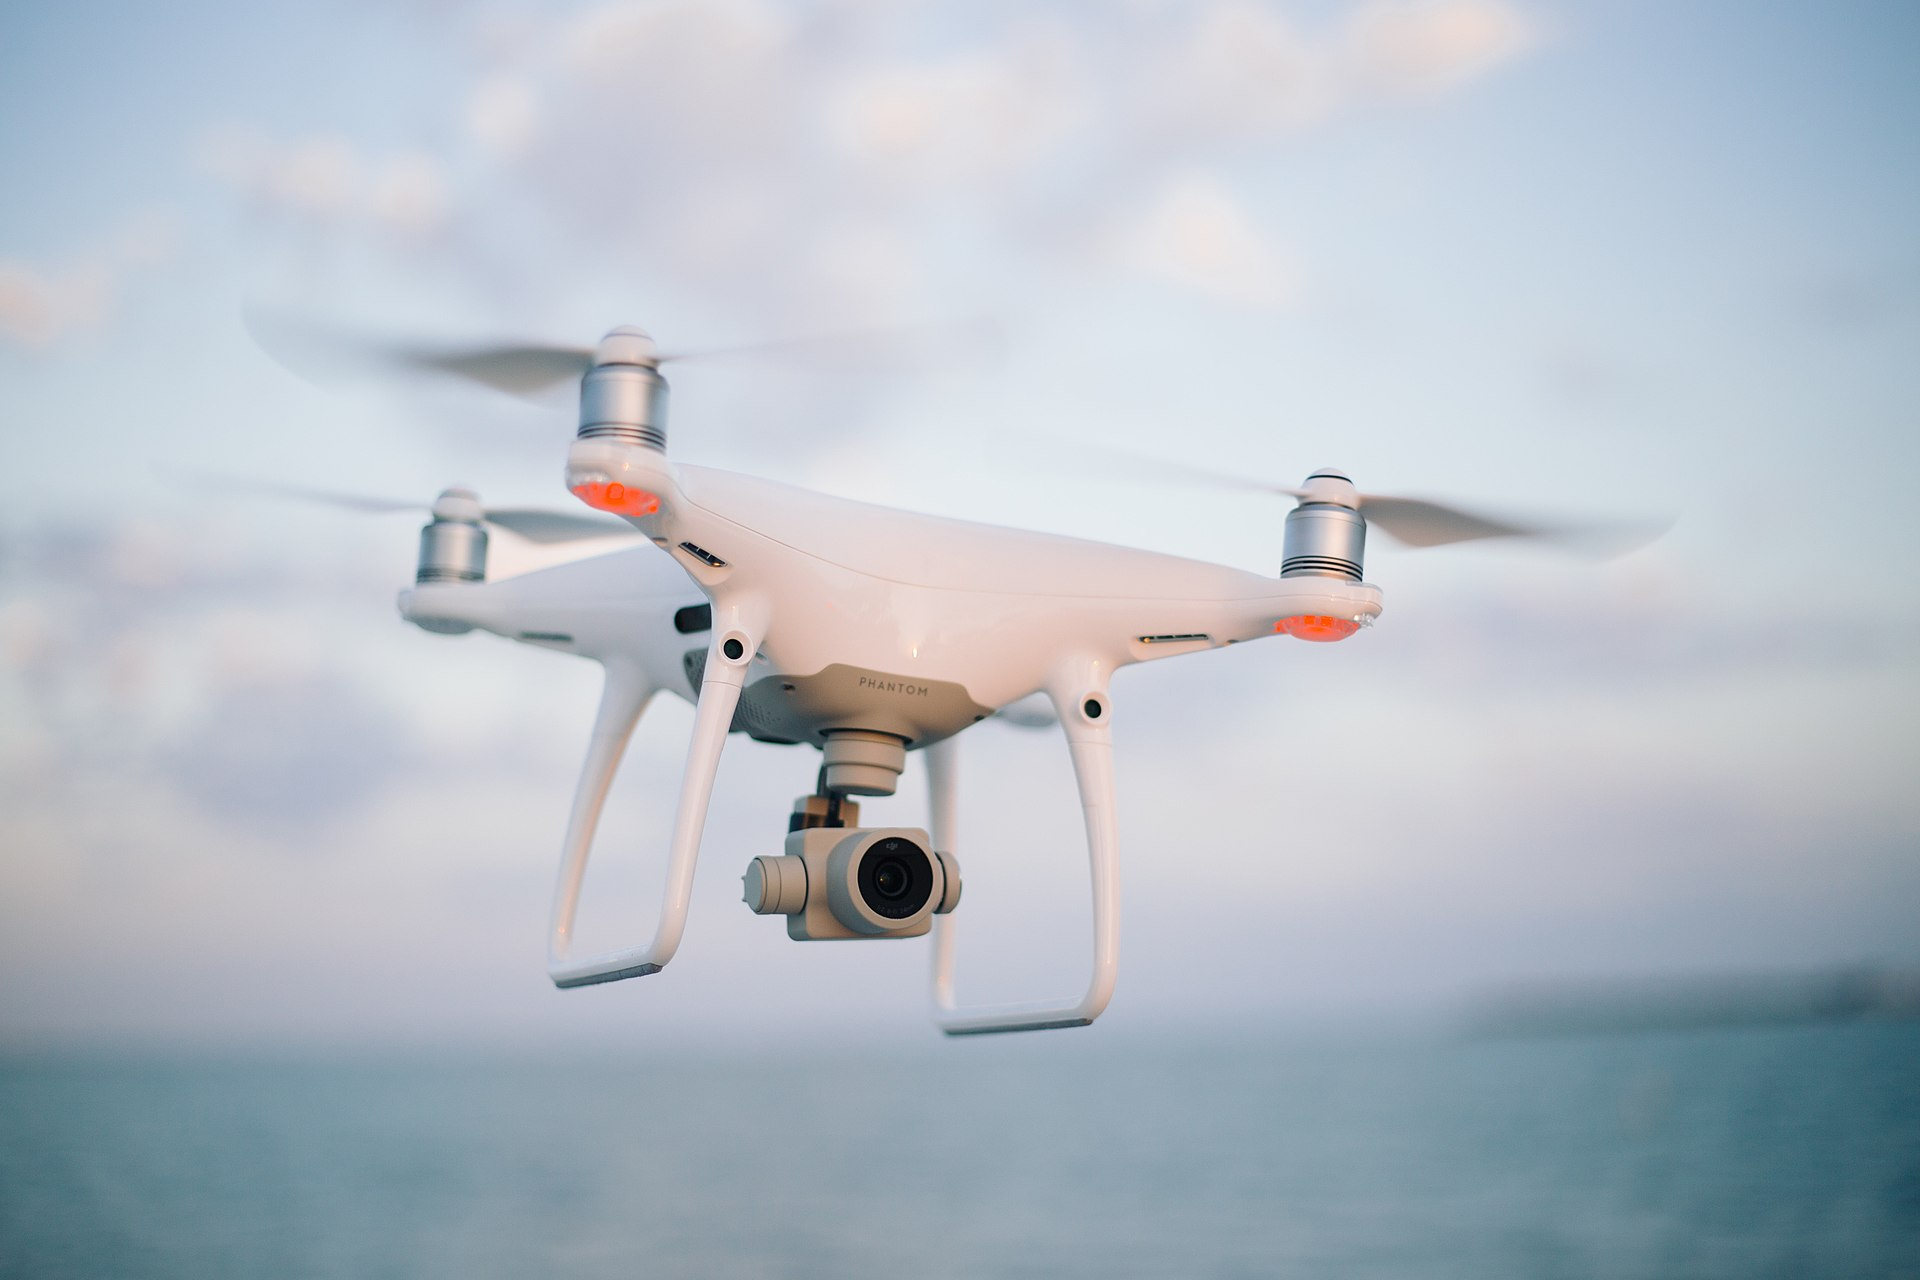
\includegraphics[width=\textwidth]{Images/Introduction/drone}
         \caption[Caption for LOF]{A DJI Phantom quadcopter (UAV)\protect\footnotemark}
         \label{fig:drone}
     \end{subfigure}
     \hfill
     \begin{subfigure}[b]{0.45\textwidth}
         \centering
         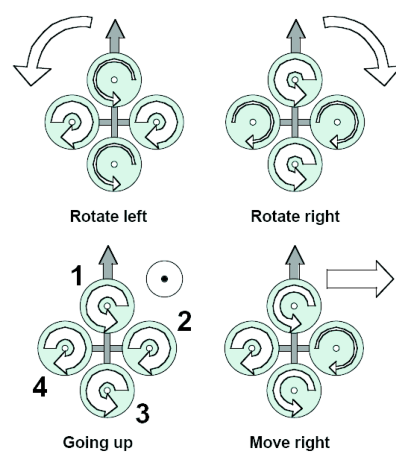
\includegraphics[width=0.6\textwidth]{Images/Introduction/propeller_direction.svg}
         \caption{Representation of the concept of a quadrotor. The width of the arrows is proportional to the angular speed of the propellers.\cite{Bouabdalla2007}}
         \label{fig:propeller_directions}
     \end{subfigure}
        \caption{A commercial quadrtotor platform with a representation of the quadrotor concept.}
        \label{fig:three graphs}
\end{figure}

\noindent The distinctive mechanical design of the quadrotor permits the actuation system to control all of the six degrees of freedom even though it is under-actuated. This is due to the fact that the rotational and translational dynamics are tightly coupled. Thus, all the translational and rotational motions can be carried off by properly controlling the magnitude and direction of the spinning speed of the rotors.   

\noindent \footnotetext[1]{\url{https://en.wikipedia.org/wiki/Quadcopter\#/media/File:Quadcopter_camera_drone_in_flight.jpg}, accessed on 01/08/2021.}


\pagebreak

Over the last few years, quadrotors have gained a large popularity in academia and in the industry. This is due to several reasons, such as: 

\begin{enumerate}

    \item Quadrotors are very simple to design and they can be easily assembled using relatively cheap components.  
    \item As quadrotors became more and more affordable and dependable, the number of real-world applications for quadrotors  has grown significantly. They are being used for aerial photography, agriculture, surveillance, inspection tasks, in addition to many other uses as well. 
    \item Quadrotors are quite agile and maneuverable during flight, especially when compared to other types of UAVs.
    
\end{enumerate}

However, one of the main challenges in the quadrotors community is the capability to design control and planning methods that will allow the quadrotors to carry out aggressive maneuvers.  The fast dynamics associated with typically small dimensions of such agile quadrotors, along with several aerodynamic effects that will become crucial during aggressive flight maneuvers, are just a few of the main problems that are faced during the system control design. Moreover, accurate tracking of the provided trajectory is a big issue in the case of aggressive maneuvers when the rotors are commanded high speeds and accelerations, which will cause rotors to become saturated and may also cause delays.


 \section*{Parallel manipulators}

A parallel manipulator is a mechanical system that consists of two connected platforms, the fixed platform and the moving platform. The latter is linked to the fixed platform thanks to at least two serial chains that are working in parallel. When compared to serial manipulators, parallel manipulators are more accurate and rigid. In addition, the ability to install the motors next to the fixed platform is a very important feature for them. Moreover, parallel manipulators can be used in a wide variety of applications that demand precision and high payload combined with high speed.\cite{Parallel_Manipulators}

\begin{figure}[h]
     \centering
     \begin{subfigure}[h]{0.45\textwidth}
         \centering
         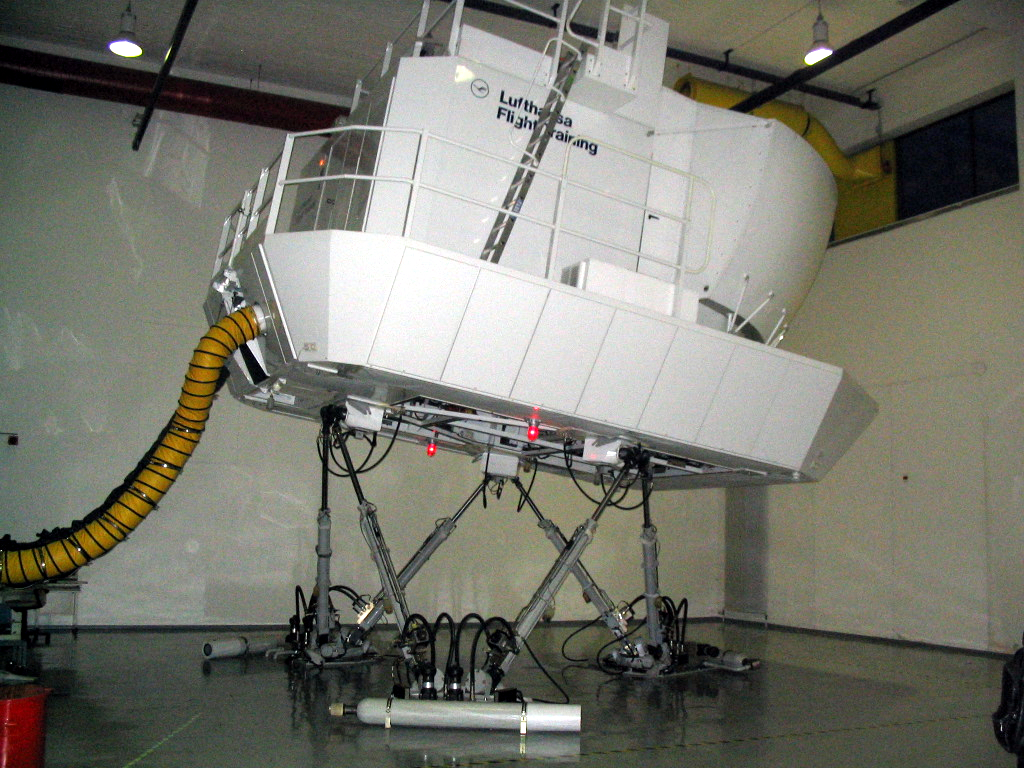
\includegraphics[width=0.7\textwidth]{Images/Introduction/GS}
    \caption[Caption for LOF]{Gough-Stewart used for a flight-simulator application.\protect\footnotemark}
         \label{GS}
     \end{subfigure}
     \hfill
     \begin{subfigure}[h]{0.45\textwidth}
         \centering
         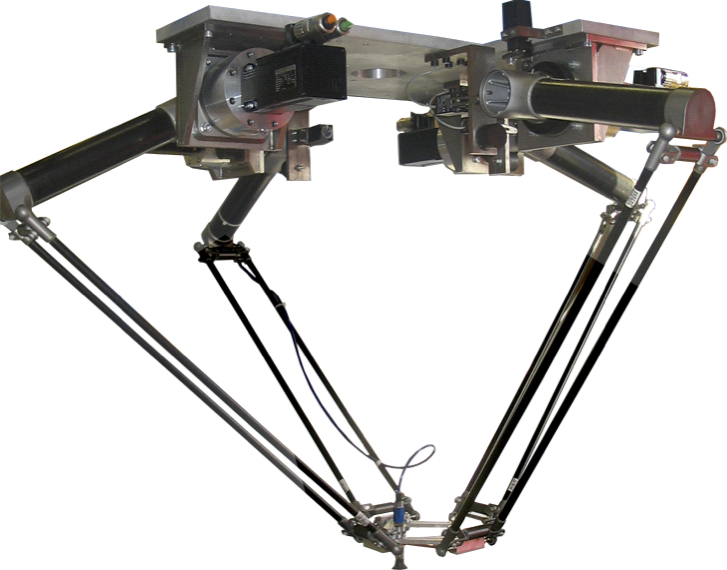
\includegraphics[width=0.7\textwidth]{Images/Introduction/PAR4}
         \caption[Caption for LOF]{The "PAR4" 4 degrees of freedom, high-speed, parallel robot prototype.\protect\footnotemark}
         \label{PAR4}
     \end{subfigure}
        \caption{Two examples of parallel robots.}
        \label{fig:three graphs}
\end{figure}




\footnotetext[1]{\url{https://en.wikipedia.org/wiki/Stewart_platform\#/media/File:Simulator-flight-compartment.jpeg}, accessed on 01/08/2021.}
\footnotetext[2]{\url{https://en.wikipedia.org/wiki/Parallel_manipulator\#/media/File:Prototype_robot_parall\%C3\%A8le_PAR4.jpg}, accessed on 01/08/2021.}


\pagebreak

However, parallel manipulators are subject to singularities which can lead to big problems in the robot workspace in case they were not handled correctly. Thus, the study of the singular configuartions of parallel manipulators is very important. Because, even just before reaching a singularity, the performance of the parallel manipulator will decrease dramatically. Moreover, the robot may loose the ability of moving in a certain direction, gain uncontrollable motions and the mechanism could even break. The main difference between serial and parallel manipulators is that singularity configurations may also appear inside the workspace of the robot (depending on the dimensions of the robot) and not just at the boundaries of the robot workspace, which can significantly decrease the area of the robot workspace.
As a result, many works have been developed by robotics researchers in order to allow parallel manipulators to safely cross these singularities by using trajectory planning and specific control methods.

\section*{The goal of this thesis}

This master thesis lies at the intersection of parallel robotics and aerial robotics. The two fields may seem very different from each other. However, quadrotors can be seen as a particular case of a parallel manipulator. 
In fact, a parallel manipulator is made up of a wrench system, applied by the robot limbs on the moving platform. And, this wrench system will define the motion of the moving platform. In the same manner, each propeller in a quadrotor can be considered as a limb of a parallel robot and the moving platform to be controlled can be considered as the body of the drone. 
Specifically, the goal of this master thesis is to study a distinct class of aggressive maneuvers for quadrotors, namely flip maneuvers. By doing flip maneuvers, full rotations around one or more axes of the body of the quadrotor can be done. In addition, the quadrotor should also be able to perform the flip maneuvers in constrained environments.

\begin{figure}[h]
     \centering
     \begin{subfigure}[h]{0.45\textwidth}
         \centering
         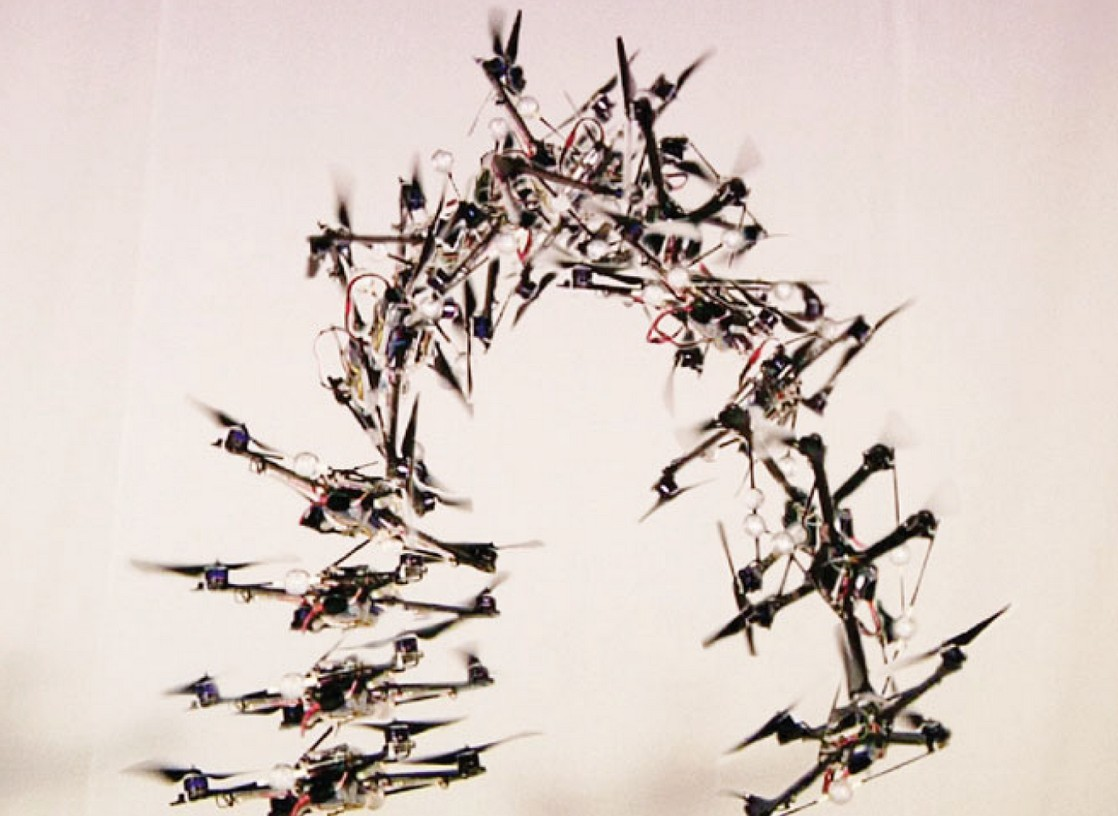
\includegraphics[width=0.9\textwidth]{Images/Introduction/flip}
    \caption{Quadrotor performing a triple flip.\cite{DAndrea2012}}
         \label{triple_flip}
     \end{subfigure}
     \hfill
     \begin{subfigure}[h]{0.45\textwidth}
         \centering
         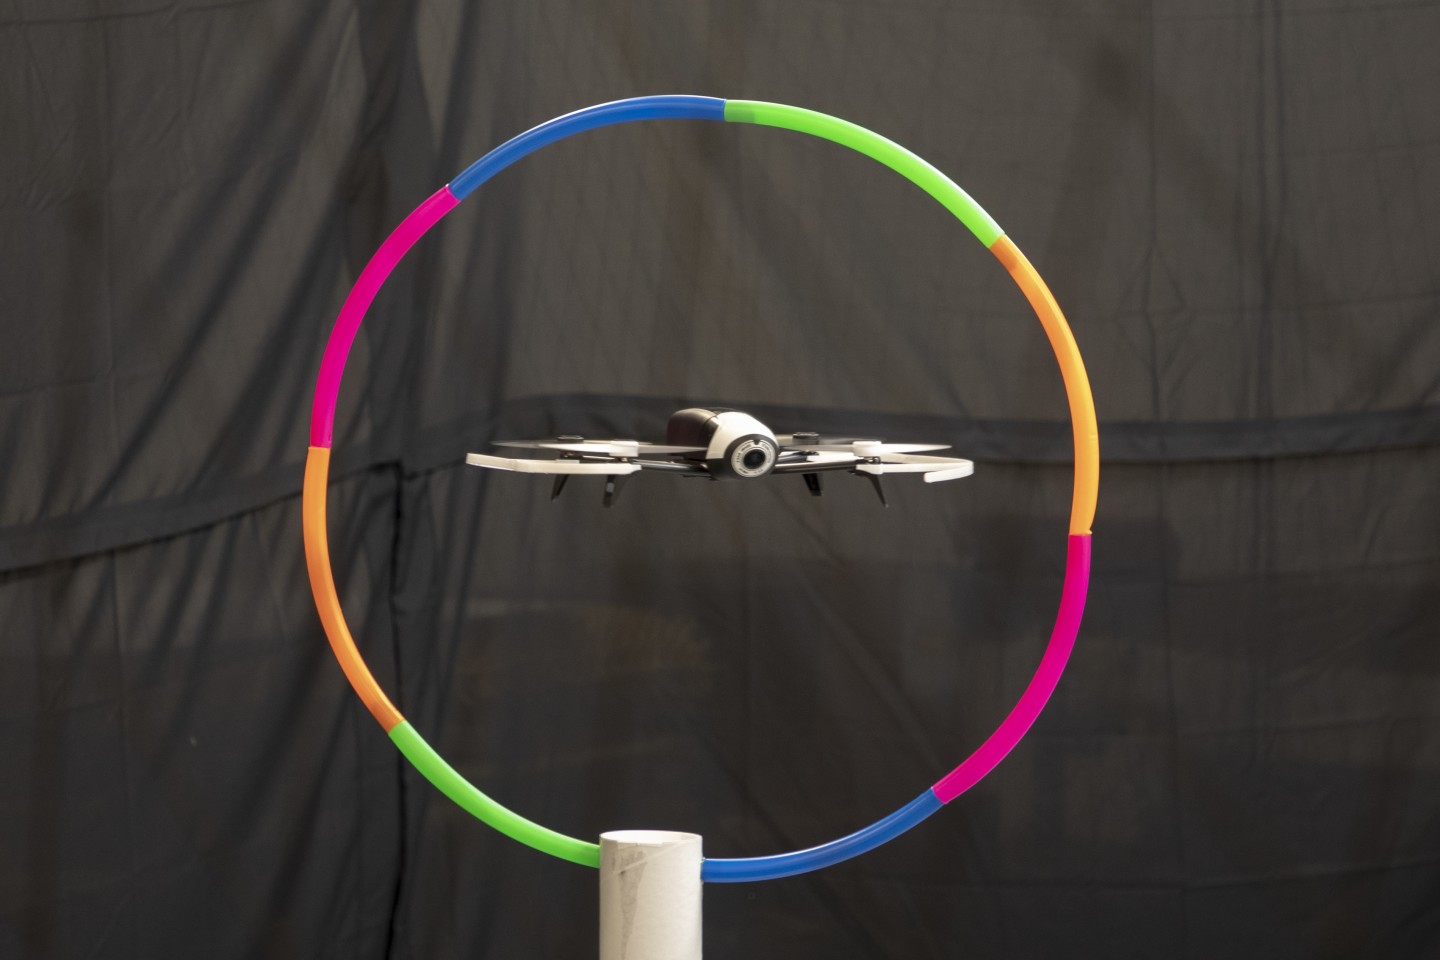
\includegraphics[width=\textwidth]{Images/Introduction/constrained_environment}
         \caption[Caption for LOF]{Quadrotor going though a loop.\protect\footnotemark[1]}
         \label{drone_hulahoop}
     \end{subfigure}
        \caption{Representation of the issues to be tackled in the master thesis.}
        \label{fig:three graphs}
\end{figure}

\footnotetext[1]{\url{https://newatlas.com/drones/muscle-signals-drone-control/\#gallery:2}, accessed on 01/08/2021.}

\pagebreak

\section*{Outline of the work}

The rest of the report is structured as follows:

\begin{comment}
\begin{itemize}
\setlength{\itemindent}{-.5in}
	\item [] \textbf{Chapter 1} is devoted to introduce the system modeling of quadrotors. Specifically, a simplified dynamic model of the quadrotor will be presented by using Euler-Lagrange formalism. Then, moving on from the simple dynamic model, a more detailed dynamic model will be presented by using the Newton-Euler formalism. Finally, the state-space model of the quadrotor will be derived.

	\item [] \textbf{Chapter 2} provides an overview of state of the art in quadrotor control in addition to introducing the different potential control methods that can be used during the master thesis in order to properly control the quadrotor. 

	\item [] \textbf{Chapter 3} provides detailed explanations of how multi-flip maneuvers can be handled. Then, the link between a quadrotor performing a flip and a parallel robot crossing a singularity will be explained. In the end, a literature review is provided in order to show how the problem is tackled by different researches.

	\item [] \textbf{Chapter 4} is devoted to trajectory optimization. By using trajectory optimization, it will be possible to create feasible trajectories for quadrotors to perform the aggressive maneuvers in constrained environments.
	
\end{itemize}
\end{comment}

\begin{itemize}
\setlength{\itemindent}{-.5in}
	\item [] \textbf{Chapter 1} provides an overview of the state of the art in the control of quadrotors and will later on focus on the main control method that will be used, namely Model Predictive Control (MPC). Moreover, a literature review of MPC applications on quadrotors will be presented. Furthermore, an overview on the software used to design a MPC controller will be presented. Finally, the state of the art in flipping maneuvers will be presented.
	
	 \item [] \textbf{Chapter 2} provides a detailed explanation of the quadrotor dynamics for the planar (2D) and 3D quadrotors. Morever, an Extended Kalman Filter (EKF) is then designed for the planar quadrotor case to be used in the presence of noisy measurements (states) and noisy control inputs. Finally, simulation results using MPC to reach a single waypoint and to follow circular trajectories with and without noise are presented.
	 
	 \item [] \textbf{Chapter 3} focuses on the trajectory generation of a flip trajectory where different optimization problems with different objective functions and initial conditions will be used in order to find the optimal flipping trajectory that satisfies the dynamic constraints of the quadrotor which will be used in the experimentation phase. Moreover, simulations with a MPC are then performed using the optimal flip trajectory.
	 
	 \item [] \textbf{Chapter 4} focuses on the simulations that were performed using ROS2 and Gazebo, in addition to the experimentation results.
\end{itemize}


\newpage
 
 \chapter{State of the art}
 
 \section{First topic}
 
 \section{Second topic}
 
 \chapter{Actual work}
  
 
 When dealing with rectangled triangles (see Figure \ref{triangle}) I sometimes used this theorem from \cite{pythm001}:
 \begin{equation}\label{theo}
  a^2 + b^2 = c^2
 \end{equation}The demonstration is in Appendix \ref{sec:prooftheorem}.
 
 \begin{figure}[h]\centering
  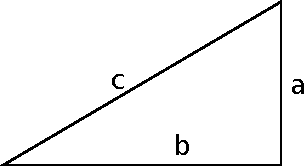
\includegraphics[width=.5\linewidth]{triangle1}
  \caption{A triangle with letters} \label{triangle}
 \end{figure}
 
 


 
 
 \chapter{Experiments}
 
 When trying to draw a rectangled triangle, my program comes up with Figure \ref{triangle2} that is neither rectangled nor a triangle.
 
  \begin{figure}[h]\centering
  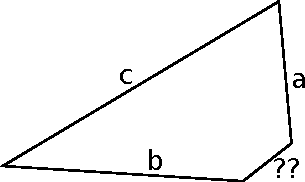
\includegraphics[width=.5\linewidth]{triangle2}
  \caption{Triangle drawn by my program. Note the 4th side.} \label{triangle2}
 \end{figure}
 
Unless there is a bug in my program, which is unlikely, this research indicates that the whole theory on triangles having 3 sides has been wrong for years, maybe decades.
 
 \chapter*{Conclusion}
 \addcontentsline{toc}{chapter}{Conclusion}
 
 
 
 
 
 % switch to A-B-C chaptering
 \appendix	
 
 \chapter{Proof of theorem \ref{theo}}
 \label{sec:prooftheorem}
 
 
 \begin{proof}
\eqref{theo} was already demonstrated in \cite{euclides300}.
\end{proof}
 
 \addcontentsline{toc}{chapter}{Bibliography}
 
 \bibliography{../biblio}
 
 
 
 
\end{document}
